\section{Training}
\label{sec:training_of_the_cnn:training}
% \todo[inline]{layout, citations, todos, cleanup, \linebreak}

% training is done in epochs (all frames from the training split are used for one epoch)
The actual training of the \acrlong{cnn} model is implemented in the Python script \texttt{cnn.py} and uses the high-level Keras \acrshort{api} from the \texttt{tf.keras} module \cite{training_arch_tf_keras}.
Four main steps are required to train the model:

\begin{enumerate}
  \item Defining the architecture (as shown in section \ref{subsec:training_of_the_cnn:architecture:implementation})
  \item Loading the training and validation datasets
  \item Compiling the model
  \item Fitting the model
\end{enumerate}

% talk about seeding % todo: cite https://www.tensorflow.org/api_docs/python/tf/random/set_seed
% or probably do not mention that since it seems to not be working
The first step is the definition of the \acrshort{cnn} architecture explained in section \ref{subsec:training_of_the_cnn:architecture:implementation}.

% The training and validation datasets are loaded with the help of the \texttt{Dataset\_Generator} class.
% The second step is the loading of the training and validation datasets, which is done with the help of the \texttt{Dataset\_Generator} class.
% The second step is the loading of the training and validation dataset splits.
% The second step is the loading of the training and validation datasets.
The second step is to load the training and validation datasets.
Since there are so many frames in the datasets, the frames are loaded in batches of \num{32} (see section \ref{subsec:training_of_the_cnn:dataset:splitting}).
% talk about the btaches of 32 and how they are loaded (Dataset_Generator from the fhnwtoys package)
% do not fit in memory
% as described in section \ref{subsec:training_of_the_cnn:dataset:splitting}.
% Furthermore, the frames are converted to the 32-bit floating-point format 
The pixel values of the frames are then converted to a 32-bit floating-point format, which is necessary for the training and further increases the required memory by a factor of \num{4}.
% talk about why the normalization is necessary
% Furthermore, the pixel values have to be normalized to the range between \numrange{0}{1}.
% Furthermore, to avoid unexpected behaviour during training, the pixel values have to be normalized to the range between \numrange{0}{1}.
To avoid unexpected behaviour during training, the pixel values have to be normalized to the range between \numrange{0}{1} \cite{training_train_scaling}.
% maybe cite this (or the other one): https://machinelearningmastery.com/how-to-normalize-center-and-standardize-images-with-the-imagedatagenerator-in-keras/

% which is done with the help of the \texttt{Dataset\_Generator} class (see listing \ref{lst:dataset_generator_class}).
This is done with the help of the \texttt{Dataset\_Generator} class.
The \texttt{Dataset\_Generator} class inherits from the \texttt{tf.keras.utils.Sequence} superclass.
The constructor loads the entire labels NumPy array and intializes the attributes of the class.
Every \texttt{tf.keras.utils.Sequence} must implementt the \texttt{\_\_len\_\_} and \texttt{\_\_getitem\_\_} methods \cite{training_arch_tf_keras_sequence}.
The \texttt{\_\_len\_\_} method returns the total number of batches when the build-in Python \texttt{len} function is called.
The \texttt{\_\_getitem\_\_} method loads a batch of frames as a NumPy array, converts the datatype to \texttt{np.float32} and normalizes the pixel values to the range between \numrange{0}{1}.
The normalization is done by dividing all pixel values by the largest possible pixel value of \num{255}.
After the normalization, the labels array is split accordingly and the batch of normalized frames and labels is return as a tuple.
The \texttt{\_\_getitem\_\_} method is invoked when the indexing operator \texttt{[]} is used on an object.
The definition of the \texttt{Dataset\_Generator} class is shown in listing \ref{lst:dataset_generator_class} and the instantiation of the dataset objects is shown in listing \ref{lst:model_fitting} on line \ref{lst:ln:training_dataset} and \ref{lst:ln:validation_dataset}.
% The dataset objects are instantiated in listing \ref{lst:model_fitting} on line \ref{} and \ref{}.
% The instantiation of the dataset objects is shown in listing \ref{lst:model_fitting} on line \ref{lst:ln:training_dataset} and \ref{lst:ln:validation_dataset}.

\begin{lstlisting}[style=python, caption={\texttt{Dataset\_Generator} class}, label=lst:dataset_generator_class]
class Dataset_Generator(utils.Sequence):
  def __init__(self, frames_name, labels_name, directory, num_batches,
               batch_size):
    self.frames_name = frames_name
    self.labels = np.load(directory / f'{labels_name}.npy')
    self.directory = directory
    self.num_batches = num_batches
    self.batch_size = batch_size

  def __len__(self):
    return self.num_batches

  def __getitem__(self, idx):
    start = idx * self.batch_size
    end = start + self.batch_size

    name = f'{self.frames_name}_batch_{idx}_of_{self.num_batches}.npy'
    frames = np.load(self.directory / name)

    batch_x = frames.astype(np.float32) / 255.0
    batch_y = np.asarray(self.labels[start:end])

    return batch_x, batch_y
\end{lstlisting}

\begin{lstlisting}[style=python, caption={Training of the model}, label=lst:model_fitting]
# 2. Loading the datasets
training_dataset = fh.Dataset_Generator((*\label{lst:ln:training_dataset}*)
  fh.training_frames_name, fh.training_labels_name,
  fh.dir_training_dataset, 4903, 32)
validation_dataset = fh.Dataset_Generator((*\label{lst:ln:validation_dataset}*)
  fh.validation_frames_name, fh.validation_labels_name,
  fh.dir_validation_dataset, 1050, 32)

# 3. Compile the model
model.compile((*\label{lst:ln:compile}*)
  optimizer='adam',
  loss=tf.keras.losses.SparseCategoricalCrossentropy(from_logits=True),
  metrics=['accuracy'])

# Save only the weights after each epoch
cp_callback = tf.keras.callbacks.ModelCheckpoint(
  filepath=str(fh.dir_checkpoint / 'cp-{epoch:04d}.ckpt'),
  save_weights_only=True,
  verbose=1,
  save_freq='epoch')

# 4. Fit the model
history = model.fit((*\label{lst:ln:fit}*)
  x=training_dataset,
  epochs=10,
  validation_data=validation_dataset,
  callbacks=[cp_callback])
\end{lstlisting}

% In a third step, the \acrshort{cnn} model is compiled, which configures the model for training \cite{}. % todo: cite https://www.tensorflow.org/versions/r2.2/api_docs/python/tf/keras/Sequential#compile
In a third step, the \acrshort{cnn} model is compiled, which configures it for training \cite{training_arch_tf_keras_sequential}.
% For this reason, an optimizer and loss function are specified.
For this reason, an optimizer, a loss function and desired metrics to evaluate are specified.
% The Adam optimizer is used, as it is computationally efficient and able to handle a large amount of parameters \cite{}. % todo: cite https://arxiv.org/pdf/1412.6980.pdf
The \textit{Adam} optimizer is used, as it is computationally efficient and can handle a large number of parameters \cite{training_arch_adam}.
% or maybe cite this, but I do not think so: https://www.tensorflow.org/versions/r2.2/api_docs/python/tf/keras/optimizers/Adam
The cross-entropy loss function is used to evaluate how well the data is modeled.
Therefore, it calculates the cross-entropy between the probability distribution of the predictions and the true labels \cite{training_train_entropy}. 
% or https://machinelearningmastery.com/cross-entropy-for-machine-learning/
Keras provides the required implementation with the \texttt{SparseCategoricalCrossentropy} class.
% The \textit{Sparse} indicates that the lables have to be provided as integers, rather than a one-hot representation.
The \textit{Sparse} indicates that the labels must be provided as integers rather than in a one-hot representation.
% Additionally, the \textit{Categorical} indicates that this is a multiclass calssification problem, rather than a binary one.
Additionally, the \textit{Categorical} indicates that it is a multiclass calssification problem and not a binary one \cite{training_train_tf_keras_crossentropy}.
% The implementation is shown in listing \ref{lst:model_fitting} on line \ref{lst:ln:compile}.
The method call is shown in listing \ref{lst:model_fitting} on line \ref{lst:ln:compile}.

% talk about epochs
% weights are updated after each batch
The last step is the fitting of the model, which is done in so-called epochs.
During an epoch, the entire dataset is used to train the model.
% The weights are updated after each batch \cite{}. % todo: cite https://www.tensorflow.org/versions/r2.2/api_docs/python/tf/keras/Sequential#fit
The training is performed batch-wise, which means that the weights are only updated after considering an entire batch \cite{training_arch_tf_keras_sequential}.
% The implementation uses a total of ten epochs ans saves the weights after each epoch (see listing \ref{lst:model_fitting} on line \ref{lst:ln:compile}).
The implementation saves the weights after each of the ten epochs (see listing \ref{lst:model_fitting} on line \ref{lst:ln:fit}).

% talk about the time it takes to train for one epoch
% with AND wihout GPU support
% explain the used GPU as well as the compute capability:
% physical GPU (device: 0, name: Quadro P3200, pci bus id: 0000:01:00.0, compute capability: 6.1)
% talk about CUDA
% todo: cite https://www.tensorflow.org/install/gpu / https://developer.nvidia.com/cuda-gpus
% The training of the \acrshort{cnn} model is performed on a decent laptop computer featuring an Intel\textsuperscript{\textregistered} Core\textsuperscript{\texttrademark} i7-8850H processor with a max. turbo frequency of \SI{4.30}{GHz}, a mobile NVIDIA Quadro P3200 graphics card with \SI{6}{GiB} of dedicated \acrshort{gpu} memory and \SI{48}{GiB} of \acrshort{ram}.
The training of the \acrshort{cnn} model is performed on a decent laptop computer featuring an Intel Core i7-8850H processor with a max. turbo frequency of \SI{4.30}{GHz}, a mobile NVIDIA Quadro P3200 graphics card with \SI{6}{GiB} of dedicated \acrshort{gpu} memory and \SI{48}{GiB} of \acrshort{ram}.
The NVIDIA Quadro P3200 \acrshort{gpu} is CUDA-enabled and features a compute capability of \num{6.1} (which currently ranges from \numrange{2.0}{8.0}).
As a result, the CUDA toolkit allows the training process to take advantage of \acrshort{gpu} acceleration \cite{training_train_nvidia}.
% Compute capabilities range from \numrange{2.0}{8.0}.

The training of a single epoch takes about \SI{76}{min} on the \acrshort{cpu} and about \SI{6}{\min} on the \acrshort{gpu}.
% This is a speedup of about  times.
This is a speedup of over $12\times$ when using the graphics card compared to the processor.

\subsection{Training Results}
\label{subsec:training_of_the_cnn:training:training_results}
% subsection results / fitting
Figure \ref{fig:training_results} shows the classification accuracy of the training and the validation dataset after each of the ten epochs.
% explain that it converges increadibly quickly
% -> thus no hyperparameter changes are necessary (like number of epochs, )
% It is evident that the accuracy converges extremely fast and thus no hyperparameter changes are required.
It is evident that the accuracy converges extremely fast, which is probably due to the ideal conditions (e.g. consistent background, good lighting).
% This is probably due to the ideal 
For this reason, no hyperparameter changes (e.g. number of epochs, batch size) are required.

The final classification accuracy is \num{0.993} for the training split and \num{0.996} for the validation split.
% there is no overfitting evident
This shows that there is no overfitting and that the \acrshort{cnn} model generalized well.

% plot of the training accuracy and the validation accuracy
\begin{figure}
  \centering
  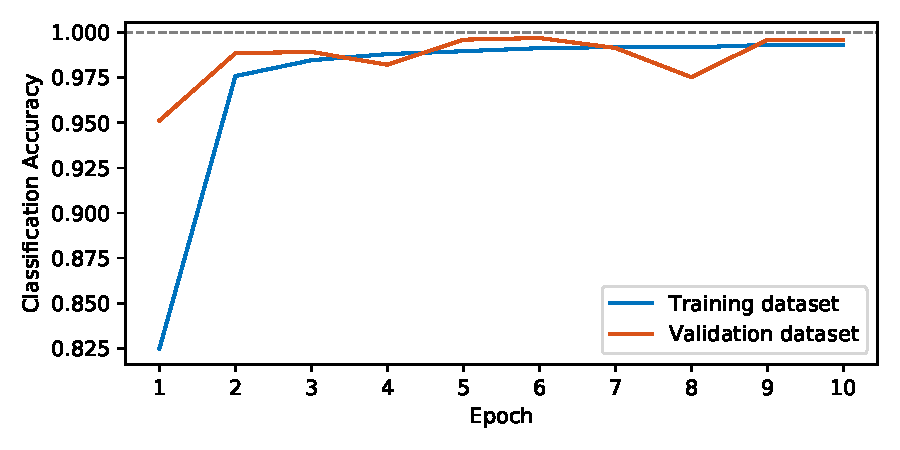
\includegraphics[width=\textwidth]{training_results}
  \caption{Results of the training of the \acrshort{cnn} model}
  \label{fig:training_results}
\end{figure}

\subsection{Saving of the Model}
\label{subsec:training_of_the_cnn:training:saving_of_the_model}
% explain the saving process of the model and the different formats they are saved in .pb / .hdf5 / frozen_graph
% The final model fit is saved in the TensorFlow SavedModel file format (\texttt{saved\_model.pb}).
The final model fit is saved in the TensorFlow SavedModel file format (\texttt{assets/}, \texttt{variables/}, \texttt{saved\_model.pb}), which includes the weights and the computation (e.g. architecture, optimizer state).
% This file format includes the weights and the computation (e.g. architecture, optimizer state), which is useful for sharing and deploying.
This is very useful for sharing and deploying of the \acrshort{cnn} model \cite{training_train_tf_keras_saving_loading}.
% this is a worse citation than the keras one % todo: cite https://www.tensorflow.org/guide/saved_model

% In addition to the 
% Inference tasks commonly use frozen graphs (single \texttt{.pb} file).
Inference tasks commonly use the frozen graph file format (single \texttt{.pb} file), which contains the architecture and the weights.
Xilinx requires such a frozen graph for the quantization of the \acrshort{cnn} model.
% Xilinx requires the model in the frozen graph file format (single \texttt{.pb} file) for .
Unfortunately, TensorFlow dropped support for freezing models since v2.x.
It is, however, still possible to freeze a model created with TensorFlow 2 with the usage of low-level TensorFlow \acrshort{api} calls.
% For this purpose
Listing \ref{lst:frozen_graph} shows how the the \texttt{frozen\_graph.pb} file is created \cite{training_train_frozen}.

For inference tasks, it is important to know the names of the input and output layers of the frozen graph.
How this information can be obtained is shown in listing \ref{lst:frozen_graph} on line \ref{lst:ln:input_info} and \ref{lst:ln:output_info}.
The name of the input layer is \texttt{x} and the name of the output layer is \texttt{Identity}.

\clearpage

\begin{lstlisting}[style=python, caption={Saving the model in the frozen graph file format \cite{training_train_frozen}}, label=lst:frozen_graph]
# Saving the frozen graph
# Convert the Keras model to a concrete function
full_model = tf.function(lambda x: model(x))
full_model = full_model.get_concrete_function(
  x=tf.TensorSpec(model.inputs[0].shape, model.inputs[0].dtype))

# Get the frozen concrete function
frozen_func = convert_variables_to_constants_v2(full_model)
frozen_func.graph.as_graph_def()

# Display information about the input and output layers
print(f'Input: {frozen_func.inputs}')(*\label{lst:ln:input_info}*)
print(f'Output: {frozen_func.outputs}')(*\label{lst:ln:output_info}*)

# Save the frozen graph from the frozen concrete function
tf.io.write_graph(
  graph_or_graph_def=frozen_func.graph,
  logdir=str(fh.dir_frozen_model),
  name='frozen_graph.pb',
  as_text=False)
\end{lstlisting}
